%! TEX root = ./master.tex
\lecture[Gruppen und Gruppenwirkungen als Kategorien. Produkt- und Funktorkategorie. Wedge- und Smash-Produkt als Funktoren. Homotopie, die Homotopiekategorie $\hTop$, Homotopieäquivalenz. Schleifen. Die Fundamentalgruppe und ihr Operator $\star$.  $\pi_1$ als Funktor $\Top_{\star} \to \Grp$]{Di 08 Jun 2021 12:15}{Homotopie}
\begin{example}\label{ex:mehr-kategorien:gruppen-produkte-wedge-smash-einhängung-funktorkategorie}
    \begin{enumerate}[1)]
        \item Wir können eine Gruppe $G$ als Kategorie auffassen, indem wir  $\Ob{\mathcat{G}} = \left \{\star\right\} $ und $\Mor_{\mathcat{G}}(\star,\star) = G$ setzen, wobei natürlich $g \circ  h = gh$. Man könnte das in etwa so skizzieren:
            \[
\begin{tikzcd}
            \bullet \ar[loop left]{}{f} \ar[loop above]{}{\id} \ar[loop right]{}{g} \ar[loop below]{}{f \circ g}
\end{tikzcd}
\]
\item Ein \vocab{G-Objekt} in einer Kategorie $\mathcat{C}$ ($G$ ist eine Gruppe) ist ein Funktor  $\mathcat{G} \to  \mathcat{C}$ (dieser Funktor besteht aus einem Objekt von $\mathcat{C}$ zusammen mit Endomorphismen dieses Objekts für jedes $g\in G$)
    \begin{remark*}
        Ein typisches Beispiel sind Gruppenwirkungen, wählen wir hier $\mathcat{C} = \Set$, so sind die $G$-Objekte genau  $G$-Mengen bzw.  $G$ wirkt dann auf die entsprechende Menge  $\mathcal{F}(\mathcat{G})\in \Set$.
    \end{remark*}
\item Sind $\mathcat{C}$, $\mathcat{D}$ Kategorien, so gibt es die \vocab{Produktkategorie} $\mathcat{C} \times  \mathcat{D}$, die wir erhalten, indem wir $\Ob{\mathcat{C} \times \mathcat{D}} = \Ob{\mathcat{C}} \times \Ob{\mathcat{D}} $ (dieses Produkt müssen wir potenziell als das von Klassen auffassen) setzen und als Morphismen
    \[
        \Mor_{\mathcat{C}\times \mathcat{D}}((X,Y),(X',Y')) \coloneqq  \Mor_{\mathcat{C}}(X,X') \times \Mor_{\mathcat{D}}(Y,Y') 
    .\] 
    setzen mit komponentenweiser Komposition, d.h. $(f,g) \circ  (f', g') = (f \circ  f', g \circ  g')$.
\item Das \nameref{def:wedge-produkt} ($\twedge$, siehe \autoref{def:wedge-produkt}) können wir nun als Funktor
     \[
    \twedge \colon \Top_{\star} \times \Top_{\star} \to  \Top_{\star}
    .\] 
    auffassen, mittels
    \[
        ((X,x_0),(Y,y_0)) \mapsto \faktor{X \coprod Y}{x_0 \sim  y_0} =\vcentcolon X \bigcup_{\left \{\star\right\} } Y 
    .\] 
    wobei der Punkt $x_0 \sim y_0$ der Basispunkt des neuen Raumes ist. Das Wedge-Produkt ist gleichzeitig auch das Koprodukt in $\Top_{\star}$.


    Analog geht das auch für das \nameref{def:smash-produkt} ($\tsmash$, siehe \autoref{def:smash-produkt}).
    \[
    \tsmash\colon  \Top_{\star} \times \Top_{\star} \to  \Top_{\star}
    .\] 
    mittels
    \[
        ((X,x_0),(Y,y_0)) \mapsto \faktor{X \times Y}{X \twedge Y}
    .\] 
    wobei wir die Einbettung
        \begin{equation*}
        \begin{array}{c c l} 
        X \twedge Y & \longrightarrow & X\times Y \\
        x & \longmapsto &  (x,y_0) \\
          & \longmapsto & (x_0,y)
        \end{array}
    \end{equation*}
    gewählt haben, um den Quotienten zu bilden, und das Bild von $X \twedge Y$ als Basispunkt von  $X \tsmash Y$ wählen.
\begin{oral}
    Das Smash-Produkt ist \emphasize{nicht} das Produkt in $\Top_{\star}$, denn dieses ist gegeben durch das übliche Produkt $X \times  Y$, wobei wir diesen Raum mittels  $(x_0,y_0) \in  X \times Y$ punktieren.
\end{oral}
\begin{minipage}{\textwidth}
    \begin{minipage}{0.7\textwidth}
        
    \begin{example}
        \begin{enumerate}[1)]
            \item $S^1 \tsmash S^1\cong S^2$ 
            \item Die \vocab{Einhängung} eines topologischen Raumes ist ein Funktor
                \[
                \Sigma \colon  \Top \to  \Top
                .\] 
                gegeben durch
                \[
                    X \mapsto \faktor{X \times [0,1]}{\substack{X\times \left \{0\right\} \\ X\times \left \{1\right\} } }
                .\] 
                (genaugenommen wollen wir hier $(x,0) \sim  (x',0)$ für $x,x'\in X$ und analog $(x,1)\sim (x',1)$ identifizieren). Für Details siehe z.B. \cite[Seite 8]{algebraic-topology-hatcher}
        \end{enumerate}
    \end{example}
    \end{minipage}
                \begin{minipage}{0.25\textwidth}
                    \centering
                    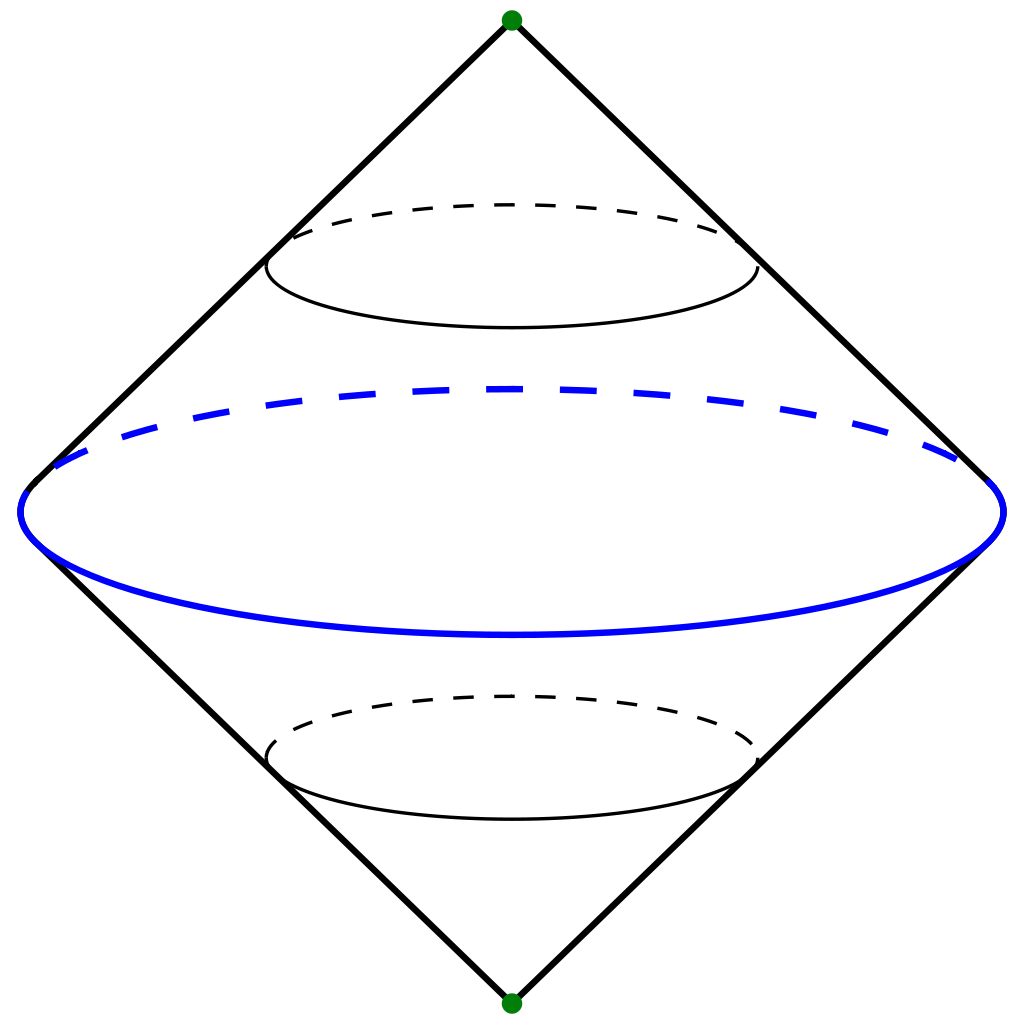
\includegraphics[width=\textwidth]{figures/1024px-Suspension.svg.png}
                    \scriptsize{Grafik von \cite{img:suspension}}
                    \captionof{figure}{Einhängung des Kreises $C^1$}
                \end{minipage}
\end{minipage}
\item Wir können die Funktorkategorie $\Mor(\mathcat{C},\mathcat{D})$ bilden, indem wir $\Ob(\Mor(\mathcat{C},\mathcat{D}))$ als die Menge der Funktoren von $\mathcat{C}$ nach $\mathcat{D}$, und $\Mor_{\Mor(\mathcat{C},\mathcat{D})}(\mathcal{F},\mathcal{G})$ als die Menge der natürlichen Transformationen von $\mathcal{F}$ nach $\mathcal{G}$ wählen.
    \end{enumerate}
\end{example}

\section{Homotopien und die Fundamentalgruppen}
\begin{oral}
    Wir reden von nun an über 'Abbildungen', wobei wir damit meinen, dass jede Abbildung automatisch stetig ist.
\end{oral}

\begin{definition}[Homotopie]\label{def:homotop}
    Zwei Abbildungen $f,g\colon  X \to  Y$ heißen \vocab{homotop}, falls es eine Abbildung
    \[
        H \colon  X \times [0,1] \to  Y
    .\] 
    gibt mit 
    \[
        H_0 \coloneqq  H(-,0) = f \qquad H_1 \coloneqq H(-,1) = g
    .\] 
    Die Abbildung $H$ nennen wir dann  \vocab{Homotopie}. 
\end{definition}

\begin{dnotation}
    Wir notieren von nun an $I \coloneqq  [0,1]$ als das Einheitsintervall.
\end{dnotation}

\begin{notation**}
    Da wir uns das Intervall $[0,1]$ als einen zeitlichen Verlauf vorstellen wollen, über dem wir  $f$ nach  $g$ homotopieren, bietet sich allgemein die Notation  $H_t \coloneqq  H(-,t) \coloneqq  X \stackrel{x \mapsto (x,t)}{\hookrightarrow} X \times [0,1] \stackrel{H}{\longrightarrow}   Y$ an, um 'die' Abbildung zum Zeitpunkt $t\in [0,1]$ zu notieren. 

    Sollte es sich bei $X$ um das Intervall  $[0,1]$ handeln, d.h.  $f,g\colon [0,1] \to  Y$ sind Wege in $Y$, so parametrisieren wir diese Wege üblicherweise mit $s$. Für Wege  $w_1,w_2$  ist dann zum Zeitpunkt $t\in [0,1]$
        \begin{equation*}
            H_t \coloneqq H(-,t)\colon  \left| \begin{array}{c c l} 
            [0,1] & \longrightarrow & Y \\
        s & \longmapsto &  H(s,t)
        \end{array} \right.
    \end{equation*}
   ein Weg in $Y$, wobei  $H_0 = w_1$ und $H_1 = w_2$.

   In der Vorlesung wir das nicht immer so gehandhabt und teilweise gewechselt, was ich persönlich verwirrend finde. Ich bemühe mich daher, einheitlich $H(s,t)$ zu verwenden und hierzu wenn nötig  $s,t$ bezüglich der Vorlesungsmitschrift zu vertauschen, damit dieses Skript einheitlich wird. Das hat den Vorteil, dass  $t$ im Kontext von Homotopien immer die Abbildungen  $X\to Y$ parametrisiert, bzw. die Notation $H_t$ die richtige ist, und - sollte es sich um Wege handeln, die wir homotopieren -  $s$ als Parameter für das Durchlaufen eines Weges verwendet wird.
\end{notation**}

\begin{lemma}
    Homotopie ist eine Äquivalenzrelation auf $\Mor_{\Top}(X,Y)$.
\end{lemma}
\begin{proof}
    \begin{description}
        \item[Reflexivität] Ist $f\colon  X \to  Y$ stetig, so auch  $H \colon  X \times I \stackrel{\pr_X}{\to } X \stackrel{f}{\to } Y $ und klarerweise ist $H_0 = H_1 = f$.
        \item[Symmetrie] Ist $H \colon  X \times I \to  Y$ stetig, so auch
            \[
                H' \colon  X \times I \stackrel{(\id, 1-t)}{\longrightarrow}  X\times I \longrightarrow  Y
            .\] 
        \item[Transitivität] Sind $H,G \colon  X \times I \to  Y$ stetig und $H_1 = G_0$, so ist auch die Abbildung
                \begin{equation*}
                HG: \left| \begin{array}{c c l} 
                X\times I & \longrightarrow & Y \\
                (x,t) & \longmapsto &  \begin{cases}
                    H(x,2t) & 0 \leq  t \leq  \frac{1}{2} \\
                    G(x, 2t-1) & \frac{1}{2}\leq t\leq 1
                \end{cases}
                \end{array} \right.
            \end{equation*}
            und wir prüfen leicht $(HG)_0 = H_0$ sowie $(HG)_1 = G_1$.
    \end{description}
\end{proof}

\begin{definition}[Homotop relativ einer Menge]\label{def:homotopie-relativ-einer-menge}
    \begin{enumerate}[i)]
        \item 
    Zwei punktierte Abbildungen $f,g \colon  (X,x_0) \to  (Y,y_0)$ heißen (punktiert) \vocab{homotop}, falls es eine Abbildung
    \[
    H \colon  X \times I \to  Y
    .\] 
    mit $H_0 = g, H_1 = g$ gibt, und zusätzlich $H_t(x_0) = y_0 \forall t\in I$ (wir lassen also den Basispunkt zu jedem Zeitpunkt fest).
\item Sei $A\subset X$ und $f,g\colon  X \to  I$. Die Abbildungen $f,g$ heißen  \vocab{homotop relativ $A$}, falls es
    \[
    H \colon  X \times I \to  Y
    .\] 
    mit $H_0 = g, H_1 = g$ und $H(a,t) = H(a,t')$ für alle  $a\in A, t\in I$ gibt (d.h, die Homotopie bleibt auf $A$ konstant). Inbesondere gilt dies nur, wenn  $f|_A = g|_A$
    \end{enumerate}
\end{definition}

\begin{definition}[Homotopiekategorie]\label{def:homotopiekategorie}
    Die \vocab{(naive) Homotopiekategorie $\hTop$}      ist die Kategorie mit $\Ob(\hTop) = \Ob(\Top)$ und 
    \[
        \Mor_{\hTop}(X,Y) = \Mor_{\Top}(X,Y) / \sim
    \]
    d.h. wir identifizieren Abbildungen modulo Homotopie.
\end{definition}

\begin{proof}
    Übung. Einige Wohldefiniertheiten müssen geprüft werden.
\end{proof}

\begin{definition}[Homotopieäquivalenz]\label{def:homotopieäquivalenz}
    \begin{enumerate}[a)]
        \item 
            Eine Abbildung $f\colon  X \to  Y$ heißt \vocab{Homotopieäquivalenz}, falls $[f]$ ein Isomorphismus in  $\hTop$ ist, d.h. falls es eine Abbildung $g\colon  Y \to  X$ gibt, so dass $g \circ  f \sim  \id_X$ und $f \circ  g \sim \id_Y$ jeweils homotop zu den Identitäten sind.
\item Existiert eine Homotopieäquivalenz $f\colon  X \to Y$, so heißen $X$ und  $Y$  \vocab{homotopieäquivalent}. 
    \end{enumerate}
\end{definition}

\begin{example}
    Der Einpunktraum $\left \{\star\right\}$ ist homotopieäquivalent zu $\R^n$ mittels
        \begin{equation*}
        f: \left| \begin{array}{c c l} 
        \left \{\star\right\}  & \longrightarrow & \R^n \\
        \star & \longmapsto &  0
        \end{array} \right.
    \end{equation*}
        \begin{equation*}
        g: \left| \begin{array}{c c l} 
        \R^n & \longrightarrow & \left \{\star\right\} \\
        x & \longmapsto &  \star
        \end{array} \right.
    \end{equation*}
    Hierbei ist $g \circ  f = \id_{\left \{\star\right\} }$ sowieso schon die Identität, und es ist $f \circ  g = \mathcal{C}_0$ (die konstante Nullabbildung). Mittels
        \begin{equation*}
        H: \left| \begin{array}{c c l} 
        \R^n\times I & \longrightarrow & \R^n \\
        (x,t) & \longmapsto &  tx
        \end{array} \right.
    \end{equation*}
    erhalten wir auch $H_0 = \mathcal{C}_0$ und $H_1 = \id_{\R^n}$, sodass wir eine Homotopie $\mathcal{C}_0 \sim \id$ gefunden haben.
\end{example}

\begin{lemma}\label{lm:homotopieäquivalenz-ist-äquivalenzrelation}
Homotopieäquivalenz ist eine Äquivalenzrelation.    
\end{lemma}

\begin{proof}
    Isomorphie in einer Kategorie ist eine Äquivalenzrelation.
\end{proof}


\begin{notation}
    Wir bezeichen
    \[
        [X,Y] \coloneqq  \Mor_{\Top}(X,Y) / \sim = \Mor_{\hTop}(X,y)
    .\] 
    und analog
    \[
        [X,Y]_{\star} \coloneqq  [(X,x_0),(Y,y_0)] \coloneqq  \Mor_{\Top_{\star}}(X,Y) / \sim 
    .\] 
\end{notation}

\begin{remark*}
    Für die Notation $[X,Y]_{\star}$ bzw. $[(X,x_0),(Y,y_0)]$ definieren wir $\sim $ natürlich wie in Teil i) von \autoref{def:homotopie-relativ-einer-menge}, d.h. wir lassen nur punktierte Homotopie zu, wie man das in der Kategorie der punktierten topologischen Räume auch erwartet, zu.
\end{remark*}

\begin{definition}[Schleife]\label{def:schleife}
    Eine \vocab[Schleife]{Schleife in $X$ an  $x\in X$} ist eine Abbildung $w\colon  I \to  X$ mit $w(0) = w(1) = x$. 

    Äquivalent ist  $w$ eine Schleife, wenn  $w\in \Mor_{\Top_{\star}}((S^1,1), (X,x_0))$, indem wir \autoref{thm:kreis-ist-quotientenraum-von-einheitsintervall} anwenden.
\end{definition}


\begin{definition}[Komposition von Schleifen]\label{def:komposition-von-schleifen}
    Für zwei Schleifen $w,w'$ in  $X$ an  $x$ ist  $w \star w'$ die Schleife mit
     \[
         (w \star w')(t) = \begin{cases}
             w(2t) & 0\leq t\leq \frac{1}{2} \\
             w'(2t-1) & \frac{1}{2}\leq t\leq 1
         \end{cases}
    .\] 
\end{definition}

\begin{theorem}\label{thm:star-ist-gruppenstruktur}
    Sei $x_0\in X$ ein Basispunkt. Dann definiert $\star$ eine Gruppenstruktur auf  $[S^1,(X,x_0)]_{\star}$.
\end{theorem}

\begin{proof}
    Als erstes zeigen wir wohldefiniertheit auf den Homotopieklassen, d.h. Wenn wir $w,w'$ bis auf Homotopie ändern, so ist auch deren Komposition bis auf Homotopie stets gleich. Seien hierzu
    \[
        H,G \colon  [0,1] / \left \{0,1\right\} \times I \to  X
    .\] 
    punktierte Homotopien. Dann setzen wir
    \[
        (H \star G)(s,t) = \begin{cases}
            H(2s,t) & 0 \leq  s \leq  \frac{1}{2} \\
            G(2s-1,t) & \frac{1}{2}\leq s\leq 1
        \end{cases}
    .\]
    und sehen sofort allgemein $(H\star G)_t = H_s \star G_t$, weswegen wir also eine Homotopie zwischen  $(H \star G)_0 = H_0 \star G_0$ und  $(H\star G)_1 = H_1 \star G_1$ definiert haben.

    Man beachte, dass wir für die Wohldefiniertheit $H(1,t) =H_t(1) =  x_0 = G_t(0) = G(0,t)$ benötigen (an der Übergangsstelle $s = \frac{1}{2}$ müssen die beiden Fälle übereinstimmen).

\begin{description}
        \item[Assoziativität] Sind $w,w',w''$ drei Schleifen an  $x_0$, so durchlaufen wir bei der Schleife $(w \star w') \star w''$ auf $[0,\frac{1}{2}]$ den Weg $w \circ  w'$ und auf $[\frac{1}{2},1]$ $w''$. Für $w \star (w' \star w'')$  passiert zwar eigentlich das Gleiche, allerdings in anderen Zeitintervallen, weswegen wir diese Zeitintervalle mittels einer Homotopie verschieben:
            \[
            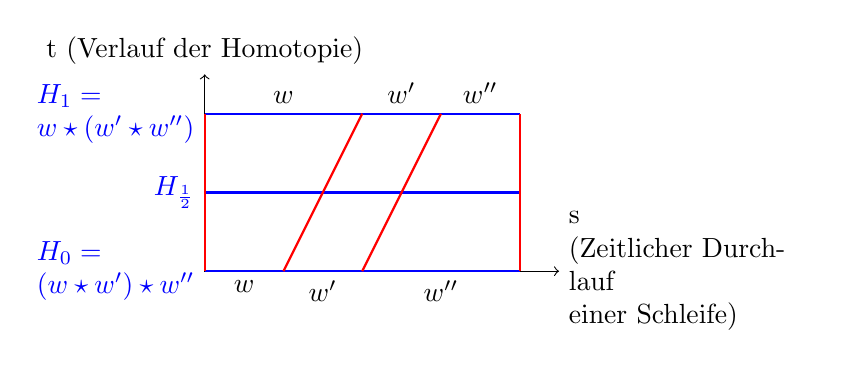
\begin{tikzpicture}
                \draw (0,0) --  (1,0) node[anchor=north, midway] {$w$} --  (2,0) node[anchor=north,midway]{$w'$} -- (4,0) node[anchor=north, midway] {$w''$} -- (4,2) -- (3,2) node[anchor=south, midway] {$w''$} -- (2,2) node[anchor=south, midway] {$w'$} -- (0,2) node[anchor=south, midway] {$w$} -- cycle;
                \draw[->] (0,0) -- (4.5,0) node[anchor=west, text width =3cm] {s \\ (Zeitlicher Durchlauf \\einer Schleife)};
                \draw[->] (0,0) -- (0,2.5) node[anchor=south] {t (Verlauf der Homotopie)};
                \draw[blue,thick] (0,2) node[anchor=east, text width=2cm] {$H_1 =$ \\ $w \star (w' \star w'')$} -- (4,2);
                \draw[blue,thick] (0,0) node[anchor=east, text width=2cm] {$H_0 =$ \\$(w \star w') \star w''$} --(4,0);
                \draw[blue,thick] (0,1) node[anchor=east] {$H_{\frac{1}{2}}$} --(4,1);
                \draw[red,thick] (2,2) -- (1,0);
                \draw[red,thick] (2,0) -- (3,2);
                \draw[red,thick] (0,0) -- (0,2);
                \draw[red, thick] (4,0) -- (4,2);
            \end{tikzpicture}
        \]
        Dazu durchlaufen wir mit $H_t$ (also zum Zeitpunkt  $t$ der Homotopie) $w$ auf dem Intervall $s\in [0, \frac{1+t}{4}]$, den Weg $w'$ auf  $[\frac{1+t}{4},\frac{2+t}{4}]$ und den Weg $w''$ auf  $[\frac{2+t}{4},1]$, formal also folgendermaßen:
    \[
        H(s,t) = \begin{cases}
            w\left( \frac{4s}{1+t} \right) & 0 \leq  s \leq  \frac{1+t}{4} \\
            w'(4s-1-t) & \frac{1+t}{4}\leq s \leq  \frac{2+t}{4} \\
            w''\left( \frac{4s-2-t}{2-t} \right) & \frac{2+t}{4}\leq s\leq 1
        \end{cases}
    .\] 
    Man prüft an den Übergängen zwischen den Wegen wieder leicht, dass für  $s = \frac{1+t}{4}$ und $s = \frac{2+t}{4}$ jeweils $H(s,t) = w(1) = x_0 = w'(0)$ bzw. $H(s,t) = w'(1) = x_0 = w''(0)$ gilt, in obiger Skizze sind die rot markierten Strecken diejenigen, auf denen $H(s,t)$ den Wert  $x_0$ (zwingend) annimmt, weil es sich um Schleifenanfänge bzw. Enden handelt.
\item[neutrales Element] Sei $c\colon  I \to X$ die Abbildung, die konstant $x_0$ ist. Wir behaupten, dass $c$ ein neutrales Elemente ist. Sei hierzu  $w$ eine beliebige Schleife an  $x$, dann ist
    \[
        H(s,t) = \begin{cases}
            w(\frac{2s}{1+t}) & 0 \leq  s\leq \frac{1+t}{2} \\
           x_0 & \frac{1+t}{2}\leq s\leq 1
        \end{cases}
    .\] 
    eine Homotopie von $w \star c$ nach  $w$. Die Abbildung $H_t$ durchläuft hierzu auf  $[0,\frac{1+t}{2}]$ den Weg $w$, und bleibt für den Rest der Zeit stehen.
    \begin{remark*}
        Wir müssen eigentlich noch zeigen, dass auch $c\star w$ zu  $w$ homotop ist, damit  $c$ eine beidseitiges neutrales Element ist, dazu ergibt sich jedoch völlig analog die Homotopie
         \[
             H(s,t) = \begin{cases}
                 x_0 & 0\leq s \leq  \frac{t}{2} \\
                 w\left( \frac{2s-t}{2-t} \right) & \frac{t}{2} \leq s \leq  1
             \end{cases}
        .\] 
        von $w$ nach  $c \star w$.  $H_t$ bleibt zunächst stehen, und durchläuft dann auf  $[\frac{t}{2},1]$ den Weg $w$.
    \end{remark*}

\item[Inverses] Sei $\overline{w} (t) = w(1-t)$, wir behaupten, dass diese Schleife ein Inverses darstellt. Dann ist
    \[
        H(s,t) = \begin{cases}
            w(2s) & 0 \leq  s \leq  \frac{1-t}{2} \\
            w(1-t) & \frac{1-t}{2} \leq  s \leq  \frac{1+t}{2} \\
            w(2-2s) = \overline{w}(2s-1) & \frac{1+t}{2} \leq  s \leq  1
        \end{cases}
    .\] 
    eine Homotopie von $w \star \overline{w}$ nach $c$. Hierbei laufen wir mit $H_t$ zunächst auf $[0, \frac{1-t}{2}]$ einen Teil von $w$ entlang (in normaler Geschwindigkeit ), dann bleiben wir stehen (an der Stelle $w(1-t)$) und laufen dann im Zeitraum  $[\frac{1+t}{2},1]$ wieder zurück, also ein Endstück von $\overline{w}$.

    \end{description}
    \begin{figure}
        \centering
        \begin{subfigure}[b]{0.15\textwidth}
            \centering
    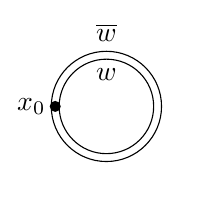
\begin{tikzpicture}[auto]
        \useasboundingbox (-1,-1) rectangle (1,1);
        \def\x{-180}
        \draw (-0.6,0) arc (180:\x:0.6) node[near start,swap] {$w$};
        \draw (-0.7,0) arc (180:\x:0.7) node[near start] {$\overline{w}$};
        \fill (-0.65,0) circle (2pt) node[anchor=east] {$x_0$}; 
        \draw (\x:0.6) -- (\x:0.7);
    \end{tikzpicture}
    \caption{$H_0$}
        \end{subfigure}
        \hfill
        \begin{subfigure}[b]{0.15\textwidth}
            \centering
    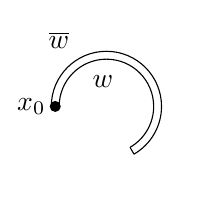
\begin{tikzpicture}[auto]
        \useasboundingbox (-1,-1) rectangle (1,1);
        \def\x{-60}
        \draw (-0.6,0) arc (180:\x:0.6) node[near start,swap] {$w$};
        \draw (-0.7,0) arc (180:\x:0.7) node[near start] {$\overline{w}$};
        \fill (-0.65,0) circle (2pt) node[anchor=east] {$x_0$}; 
        \draw (\x:0.6) -- (\x:0.7);
    \end{tikzpicture}
    \caption{$H_{\frac{1}{3}}$}
        \end{subfigure}
        \hfill
        \begin{subfigure}[b]{0.15\textwidth}
            \centering
    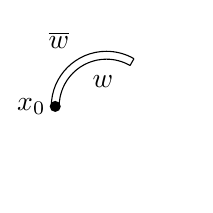
\begin{tikzpicture}[auto]
        \useasboundingbox (-1,-1) rectangle (1,1);
        \def\x{60}
        \draw (-0.6,0) arc (180:\x:0.6) node[midway,swap] {$w$};
        \draw (-0.7,0) arc (180:\x:0.7) node[midway] {$\overline{w}$};
        \fill (-0.65,0) circle (2pt) node[anchor=east] {$x_0$}; 
        \draw (\x:0.6) -- (\x:0.7);
    \end{tikzpicture}
    \caption{$H_{\frac{2}{3}}$}
        \end{subfigure}
        \hfill
        \begin{subfigure}[b]{0.15\textwidth}
            \centering
    \begin{tikzpicture}[auto]
        \useasboundingbox (-1,-1) rectangle (1,1);
        \def\x{120}
        \draw (-0.6,0) arc (180:\x:0.6) node[near end,swap] {$w$};
        \draw (-0.7,0) arc (180:\x:0.7) node[near end] {$\overline{w}$};
        \fill (-0.65,0) circle (2pt) node[anchor=east] {$x_0$}; 
        \draw (\x:0.6) -- (\x:0.7);
    \end{tikzpicture}
    \caption{$H_{\frac{5}{6}}$}
        \end{subfigure}
        \hfill
        \begin{subfigure}[b]{0.15\textwidth}
            \centering
    \begin{tikzpicture}[auto]
        \useasboundingbox (-1,-1) rectangle (1,1);
        \fill (-0.65,0) circle (2pt) node[anchor=east] {$x_0$}; 
    \end{tikzpicture}
    \caption{$H_1$}
        \end{subfigure}
        \caption{Illustration der Homotopie von $w \star \overline{w}$ zu $c$ mit dem 'Spaghetti-Trick'}
    \end{figure}
\end{proof}

\begin{oral}
    Man erkennt, dass es für obigen Beweis wichtig war, dass wir die Verknüpfung nur bis auf Homotopie definieren, weil wir ansonsten Probleme mit der Parametrisierung bekommen.
\end{oral}

\begin{definition}[Fundamentalgruppe]\label{def:fundamentalgruppe}
    Für $(X,x_0) \in \Top_{\star}$ ist 
    \[
        \pi_1(X,x_0) \coloneqq  ([(S^1,1),(X,x_0)]_{\star},\star)
    .\] 
    die \vocab{Fundamentalgruppe} von $X$ an  $x_0$. 
\end{definition}

\begin{oral}
    Wir werden feststellen, dass es sich bei obigem um eine Homotopieinvariante handelt, mit der wir eine weitere charakteristische Eigenschaft von topologischen Räumen gefunden haben, um diese zu unterscheiden. 

    Allerdings wird sich herausstellen, dass die Berechnung solcher Gruppen recht mühsam ist, weswegen wir noch die Technik sogenannter \textit{Überlagerungen} kennenlernen werden.
\end{oral}

\begin{theorem}
    Ist $f\colon  (X,x_0) \to  (Y,y_0)$ eine Abbildung, so induziert diese einen Gruppenhomomorphismus
    \[
        \pi_1 (X,x_0) \stackrel{\pi_1(f) =: f_*}{\longrightarrow}   \pi_1(Y,y_0)
    .\] 
    mittels $[w] \mapsto [f \circ  w]$. Zudem ist
    \[
    \pi_1\colon  \Top_{\star} \to  \Grp
    .\] 
    ein Funktor.
\end{theorem}

\begin{proof}
    \begin{description}
        \item[Wohldefiniertheit] Ist $w\stackrel{H}{\sim} w'$, so ist $f \circ  w \stackrel{f \circ  H}{\sim }  f \circ  w''$.
        \item[Gruppenhomomorphismus] Seien $[w], [w']$ zwei beliebige Element aus  $\pi_1(X,x_0)$, dann ist 
            \begin{IEEEeqnarray*}{rCl}
                \pi_1(f) ([w] \star [w']) &=& \pi_1(f) ([w\star w']) \\
                                        & = & [f \circ  (w \star w')] \\
                                        & \stackrel{\text{(1)}}{=}  & [(f \circ  w) \star (f \circ  w') ] \\
                                        & = & [f \circ  w] \star [f \circ  w'] \\
                                        & = & \pi(f) ([w]) \circ  \pi_1(f)([w'])
            \end{IEEEeqnarray*}
            wobei in (1) Gleichheit gilt, weil es sich bei beiden Seiten um die Abbildung
            \[
            \begin{cases}
                (f \circ w)(2t) & 0\leq t\leq \frac{1}{2} \\
                (f \circ  w') (2t-1) & \frac{1}{2}\leq t\leq 1
            \end{cases}
            .\]
            handelt. 
        \item[Funktorialität] 
            \begin{itemize}
                \item Es ist $\pi_1(\id_X) [w] = [\id_X \circ  w] = [w]$, also bilden wir Identitäten auf Identitäten ab.
                \item Wir rechnen nach:
                    \begin{IEEEeqnarray*}{rCl}
                        \pi_1(f \circ g)([w]) & = & [(f \circ g) \circ  w] \\
                                              &=& [f \circ  (g \circ  w)] \\
                                              & = & \pi_1(f) [g \circ  w] \\
                                              & = & \pi_1(f)(\pi_1(g)[w]))\\
                                              & = & (p_1(f) \circ  \pi_1(g))[w]
                    \end{IEEEeqnarray*}
                    und wir erhalten, dass $\pi_1(f \circ g) = \pi_1(f) \circ  \pi_1(g)$.
            \end{itemize}
    \end{description}
\end{proof}

\begin{oral}
    Wir können uns $\pi_1$ vorstellen als 'Löcher-zählen', dazu später mehr.
\end{oral}

